\documentclass[11pt]{article}
\usepackage[margin=1in]{geometry}
\usepackage{amsmath,amssymb,amsthm,mathtools}
\usepackage{booktabs,enumitem,graphicx,xcolor}
\usepackage{xurl}
\usepackage[colorlinks=true,linkcolor=blue!50!black,citecolor=green!35!black,urlcolor=blue!50!black]{hyperref}
\usepackage[nameinlink]{cleveref}
\graphicspath{{figs/}}

\newtheorem{theorem}{Theorem}
\newtheorem{proposition}[theorem]{Proposition}
\newtheorem{lemma}[theorem]{Lemma}
\newtheorem{corollary}[theorem]{Corollary}
\theoremstyle{definition}
\newtheorem{example}[theorem]{Example}
\newtheorem{problem}[theorem]{Open problem}
\theoremstyle{remark}
\newtheorem{remark}[theorem]{Remark}
\crefname{problem}{open problem}{open problems}

\newcommand{\EE}{\mathbb E}
\newcommand{\cx}{\le_{\mathrm{cx}}}
\newcommand{\KL}{\mathrm{KL}}
\DeclareMathOperator{\logit}{logit}

\title{Pooling Informed Agents:\\ Blackwell Order, Reconciliation and the KL Ball}
\author{V.~K. Awasthi}
\date{October 2026}

\begin{document}
\maketitle

\begin{abstract}
Several agents report posteriors about one binary state. What can be inferred from their reports, and when does pooling a less
informed agent with a more informed one help? We collect the answers in one place, with short proofs. The agents share a prior iff an
entropy term vanishes. Convex order of their posterior laws is Blackwell's information order, which mutual information totalises. Two
overlapping pairs of logs always reconcile, while three pairs can fail, with a cycle inequality as certificate. The main result
characterises the pooling rules that are at least as good as the better agent in expected log loss: they form a KL ball around the
Bayes pool whose radius is the conditional information $I(X;q_j\mid q_i)$. The radius vanishes exactly under a Beck--Chevalley
(conditional independence) condition, so for a Blackwell-garbled agent the only rule that is not worse is to ignore it, and the
Blackwell order of the two posterior laws alone cannot decide which case holds. A Pinsker-type bound turns the ball into decisions:
any rule in the ball errs at most $\sqrt{2I(X;q_j\mid q_i)}$ more often, weighted by margin, than the Bayes decision. Every statement
is checked by a script (nine checks, all passing).
\end{abstract}

\section{Setting}
A binary state $X$ has prior $P(X=1)=\rho$. Agent $i$ sees a signal $S_i$ with kernel $P(S_i\mid X)$ and reports the posterior
$q_i=P(X=1\mid S_i)$. The law $\Pi_i$ of $q_i$ is agent $i$'s \emph{tower}, with barycentre $\rho_i=\int q\,d\Pi_i$; in the language of
the companion paper \cite{Main} it is the second level of a three-level posterior tower, and the facts below are the multi-agent reading
of its martingale structure \cite[Thm.~5.3]{Main}. When agents are pooled, the agent index $Z$ is drawn with weights $w_i$. When answers
are logged, $A_i\in\{0,1\}$ is agent $i$'s binary answer. A \emph{pooling rule} $F$ maps a pair of reports to a posterior
$F(q_i,q_j)$, item by item; the \emph{Bayes pool} is $q^*=P(X=1\mid q_i,q_j)$. Losses are expected log losses,
$\mathrm{loss}(F)=\EE[-\log F(X)]$, in nats unless stated otherwise.

The checks are in \texttt{check\_agents.py} (AG1--AG9); the figure is drawn by \texttt{fig\_agents.py}.

\section{What one agent's tower says}
\begin{proposition}[Common prior]\label{prop:prior}
\begin{enumerate}[label=(\alph*)]
\item If the agents are Bayesian with common prior $\rho$, then $\rho_i=\rho$ for every $i$.
\item For pooled agents, with $\bar\rho=\sum_iw_i\rho_i$,
\[
H(\bar\rho)=\underbrace{H(\bar\rho)-\textstyle\sum_iw_iH(\rho_i)}_{I(X;Z)}+\underbrace{\textstyle\sum_iw_i\bigl(H(\rho_i)-\EE H(q_i)\bigr)}_{I(X;S_Z\mid Z)}
+\underbrace{\textstyle\sum_iw_i\,\EE H(q_i)}_{H(X\mid Z,S_Z)},
\]
and the first term vanishes iff all $\rho_i$ are equal.
\end{enumerate}
\end{proposition}
\begin{proof}
(a) $\EE q_i=\EE P(X=1\mid S_i)=P(X=1)$, Bayes plausibility \cite{KamenicaGentzkow2011}. (b) The chain rule along $Z$, then $S_Z$; equality
by strict concavity of $H$. Checks AG1, AG2.
\end{proof}

\begin{proposition}[Who knows more]\label{prop:blackwell}
Suppose $\rho_i=\rho_j$.
\begin{enumerate}[label=(\alph*)]
\item If $S_j$ is a garbling of $S_i$ (it depends on $X$ only through $S_i$), then $\Pi_j\cx\Pi_i$.
\item Conversely, $\Pi_j\cx\Pi_i$ implies that $S_j$ is equivalent to a garbling of $S_i$ \cite{Blackwell1953}.
\item $\Pi_j\cx\Pi_i$ iff $\EE(q_j-t)_+\le\EE(q_i-t)_+$ at every support point $t$ of either law \cite[Thm.~3.A.1]{ShakedShanthikumar2007};
  this is an exact finite test.
\item $\Pi_j\cx\Pi_i$ implies $I(X;q_j)\le I(X;q_i)$, but not conversely.
\end{enumerate}
\end{proposition}
\begin{proof}
(a) $q_j=\EE[q_i\mid S_j]$, a martingale coupling. (b) Blackwell's theorem. (c) Stop-loss transforms of laws on $[0,1]$ with equal means
are piecewise linear with kinks at support points. (d) $I(X;q)=H(\rho)-\EE H(q)$ and $-H$ is convex; \cref{ex:three} gives the converse.
Checks AG3, AG4.
\end{proof}

\begin{example}[Three agents with $\rho=\tfrac12$]\label{ex:three}
Agent $a$ has accuracy $0.8$, so $\Pi_a=\tfrac12\delta_{1/5}+\tfrac12\delta_{4/5}$. Agent $b$ learns $X$ with probability $0.2$ and nothing
otherwise: $\Pi_b=\tfrac1{10}\delta_0+\tfrac45\delta_{1/2}+\tfrac1{10}\delta_1$. Agent $c$ sees $a$'s signal flipped with probability
$\tfrac14$: $\Pi_c=\tfrac12\delta_{7/20}+\tfrac12\delta_{13/20}$. Then $c\prec a$, and $b$ is incomparable with both (\cref{fig:agents}a).
Mutual information still ranks them $a>b>c$ ($0.278$, $0.200$, $0.066$ bits), hiding that $b$ is certain on a fifth of the items.
\end{example}

\section{What joint logs say}
\begin{lemma}[Two windows always glue]\label{lem:glue}
Let $P_{UV}$ and $P_{VW}$ be laws of finite variables with the same $V$-marginal. Then $P=P_{UV}P_{VW}/P_V$ (with $0/0=0$) is a joint law
with both windows, and it is the only one with $U\perp W\mid V$. For full-support laws this is the Beck--Chevalley condition for the
windows $\sigma(U,V)$, $\sigma(V,W)$ \cite[Thm.~14.4]{Main}.
\end{lemma}
\begin{proof}
Summing out $w$ or $u$ returns the windows. The law factorises as $P(u\mid v)P(w\mid v)P(v)$; conversely conditional independence forces
this factorisation.
\end{proof}

\begin{proposition}[Reconciling three agents]\label{prop:glue}
Logs record the answers of agents $i,j$ on common items for some pairs; each agent's answers are calibrated with known accuracy. The logs
are \emph{feasible} if some common prior and private signals produce all of them.
\begin{enumerate}[label=(\alph*)]
\item If the pairs $\{1,2\}$ and $\{2,3\}$ are each feasible, they are jointly feasible.
\item Feasible logs for all three pairs satisfy the cycle inequalities $d_{ik}\le d_{ij}+d_{jk}$ and $d_{12}+d_{23}+d_{13}\le2$, where
  $d_{ij}=P(A_i\ne A_j)$. Without calibration these four inequalities are also sufficient; with calibration the exact test is a linear
  program over $P(X,A_1,A_2,A_3)$.
\item With accuracy $\tfrac34$ for all three agents, $d_{12}=d_{23}=\tfrac1{20}$ and $d_{13}=\tfrac12$, every pair and the chain are feasible
  but the three pairs together are not; $d_{13}\le d_{12}+d_{23}$ fails by $\tfrac25$.
\end{enumerate}
\end{proposition}
\begin{proof}
(a) Calibration and the answer rates fix the $(X,A_2)$ margin, so \cref{lem:glue} with $V=(X,A_2)$ glues the two pair laws.
(b) $A_i\ne A_k$ forces $A_i\ne A_j$ or $A_j\ne A_k$, and each outcome of $(A_1,A_2,A_3)$ has $0$ or $2$ disagreeing pairs; these four
inequalities are the facets of the cut polytope of the triangle. For many agents and the hardness of the general problem see
\cite{ArieliEtAl2021}. (c) Check AG5.
\end{proof}

\begin{proposition}[Chain pooling]\label{prop:chain}
With $X$ recorded, the chain rule
\[
\hat P(X\mid a_1,a_2,a_3)\ \propto\ \frac{P(X,a_1,a_2)\,P(X,a_2,a_3)}{P(X,a_2)}
\]
equals the true posterior when
$A_1\perp A_3\mid(X,A_2)$; for generic laws it does not. The product of independent experts, $\hat P\propto\rho\prod_iP(a_i\mid X)$,
needs the stronger mutual independence given $X$.
\end{proposition}
\begin{proof}
Under the independence the joint is the glued law of \cref{lem:glue}. Check AG6.
\end{proof}

\section{Pooling a more and a less informed agent}
\begin{theorem}[The KL ball]\label{thm:ball}
For every joint law of $(X,S_i,S_j)$ and every pooling rule $F$,
\[
\mathrm{loss}(q_i)-\mathrm{loss}(F)\;=\;I(X;q_j\mid q_i)\;-\;\EE\,\KL\bigl(q^*\,\big\|\,F(q_i,q_j)\bigr).
\]
\begin{enumerate}[label=(\alph*)]
\item $F$ is weakly better than agent $i$ iff $\EE\,\KL(q^*\|F)\le I(X;q_j\mid q_i)$, and strictly worse iff the reverse strict inequality
  holds. The good rules form a KL ball around $q^*$ of radius $I(X;q_j\mid q_i)$.
\item The radius vanishes iff $X\perp q_j\mid q_i$, which for full support is Beck--Chevalley for $\sigma(X,q_i)$ and $\sigma(q_i,q_j)$.
\item \emph{Blackwell case.} If $S_j$ is a garbling of $S_i$, then $q^*=q_i$; a rule is weakly better than $i$ only if $F=q_i$ almost
  surely, and otherwise it is worse by exactly $\EE\,\KL(q_i\|F)$.
\item The order $\Pi_j\cx\Pi_i$ alone does not decide: the radius depends on the coupling of the signals (\cref{ex:same}).
\item The same holds for every strictly proper scoring rule with KL replaced by its divergence \cite{GneitingRaftery2007}; for the Brier
  score $(X-F)^2$, $\mathrm{loss}(q_i)-\mathrm{loss}(F)=\EE(q^*-q_i)^2-\EE(q^*-F)^2$.
\end{enumerate}
\end{theorem}
\begin{proof}
Given $(q_i,q_j)$, $X$ has law $q^*$, so $\EE[-\log F(X)\mid q_i,q_j]=H(q^*)+\KL(q^*\|F)$. Subtracting the case $F=q_i$ and using
$\EE\,\KL(q^*\|q_i)=I(X;q_j\mid q_i)$ gives the identity and (a). (b) is the equality case of conditional mutual information, with the
meet of the two windows equal to $\sigma(q_i)$ under full support. (c) A garbling gives $X\perp S_j\mid S_i$, so $q^*=q_i$. (e) Replace
$H(q^*)+\KL$ by the entropy and Bregman divergence of the score. Checks AG7 (the identity and its Brier form, 300 laws $\times$ 4 rules)
and AG8 (200 garblings).
\end{proof}

\begin{example}[Same towers, different answers]\label{ex:same}
Let $\rho=\tfrac12$, agent $i$ have accuracy $0.8$ and agent $j$ accuracy $0.65$, so $\Pi_j\cx\Pi_i$. Expected log loss in bits:
\begin{center}\small
\begin{tabular}{lcccc}\toprule
coupling of the signals & $i$ alone & Bayes pool & linear pool & log pool\\\midrule
$S_j$ = $S_i$ flipped w.p.\ $\tfrac14$ (garbling) & 0.722 & 0.722 & 0.779 & 0.770\\
$S_j$ independent of $S_i$ given $X$ & 0.722 & 0.679 & 0.756 & 0.747\\\bottomrule
\end{tabular}
\end{center}
Both pools use equal weights. In the first row nothing beats $i$; in the second the Bayes pool gains $0.042$ bits, the radius, while both
equal-weight pools still lie outside the ball. Along the log-odds family $\logit F=\logit q_i+\gamma\logit q_j$ the ball is the interval
$0<\gamma<2.02$ in the second case and the single point $\gamma=0$ in the first (\cref{fig:agents}b).
\end{example}

\begin{figure}[t]\centering
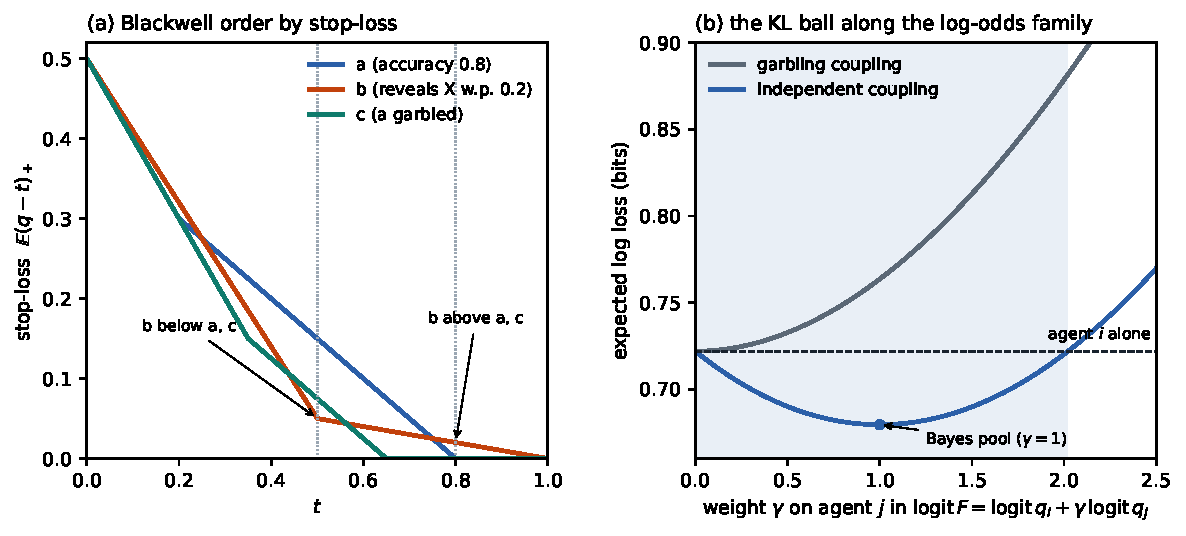
\includegraphics[width=\linewidth]{fig_agents}
\caption{(a) Stop-loss transforms of the agents of \cref{ex:three}: $c$ lies below $a$, so $c\prec a$; $b$ crosses both, so it is
incomparable with them. (b) Expected log loss of the log-odds pool against the weight $\gamma$ on agent $j$, for the two couplings of
\cref{ex:same}. The shaded band is the set of $\gamma$ for which the pool is at least as good as agent $i$ under the independent coupling;
under the garbling coupling the band shrinks to $\gamma=0$.}
\label{fig:agents}
\end{figure}

\section{From the ball to decisions}
Most uses of a pooled posterior end in a decision. Let $d_F=\mathbf 1\{F\ge\tfrac12\}$ and $d^*=\mathbf 1\{q^*\ge\tfrac12\}$, and let
$\mathrm{err}(F)=P(d_F\ne X)$. The excess error of $F$ over the Bayes decision is
\[
\mathrm{err}(F)-\mathrm{err}(q^*)=\EE\bigl[\,|2q^*-1|\;\mathbf 1\{d_F\ne d^*\}\bigr],
\]
the rate at which $F$ and the Bayes pool decide differently, weighted by how much the difference costs.

\begin{proposition}[Decision error of rules in the ball]\label{prop:decision}
For every pooling rule $F$,
\[
\mathrm{err}(F)-\mathrm{err}(q^*)\;\le\;2\,\EE|q^*-F|\;\le\;\sqrt{2\,\EE\,\KL(q^*\|F)}.
\]
Consequently every rule at least as good as agent $i$ in log loss satisfies
\[
\mathrm{err}(F)-\mathrm{err}(q^*)\ \le\ \sqrt{2\,I(X;q_j\mid q_i)},
\]
and so does agent $i$ itself. In the Blackwell case the bound is $0$.
\end{proposition}
\begin{proof}
If $d_F\ne d^*$, then $F$ and $q^*$ lie on opposite sides of $\tfrac12$, so $|2q^*-1|\le2|q^*-F|$; this gives the first inequality. For
Bernoulli laws the total variation distance is $|q^*-F|$, and Pinsker's inequality gives $|q^*-F|\le\sqrt{\KL(q^*\|F)/2}$
\cite{CoverThomas2006}; Jensen's inequality moves the expectation inside the square root. For a rule in the ball,
$\EE\,\KL(q^*\|F)\le I(X;q_j\mid q_i)$ by \cref{thm:ball}(a); agent $i$ is the case $F=q_i$. Check AG9 confirms both inequalities on 2000
random laws and the corollary on the 1268 rules among them that lie in the ball; the largest observed ratios to the bounds are $0.63$ and
$0.45$.
\end{proof}

\begin{remark}[Inversions]
The natural quantity to watch is the excess error above, not the rate at which $F$ overrides agent $i$. Overriding $i$ is often correct:
outside the Blackwell case the Bayes pool should override $i$ whenever $j$'s evidence outweighs $i$'s, and those overrides are where the
gain comes from. In \cref{ex:same} the independent agent $j$ is too weak ever to overturn $i$: all four rules make the same decisions,
with error $0.2$, although their log losses differ. The bound $\sqrt{2I}=0.24$ is then far from tight, as a worst-case bound must be.
\end{remark}

\begin{problem}[The radius over the fibre]\label{op:radius}
When only pairwise logs are available, the coupling of the signals is known only up to the set of joint laws consistent with them. Compute
the smallest and largest values of $I(X;q_j\mid q_i)$ over that set. If the largest is $0$, no consistent coupling lets $j$ help, and
every rule other than $F=q_i$ is strictly worse; if the smallest is positive, the Bayes pool helps under every consistent coupling, and by
\cref{prop:decision} its decisions are never worse than $i$'s by more than $\sqrt{2I}$.
\end{problem}

\section*{Scope}
Each agent's tower describes its uncertainty about $X$, not its beliefs about the other agents. To reason about beliefs about beliefs,
agent $1$ must report a law over agent $2$'s posteriors, which is a further tower one level up; the statements above then apply there. For
$n$ agents the cycle inequalities remain necessary, \cref{prop:glue}(a) extends to any tree of overlapping pairs, and the general
feasibility problem is hard; see \cite{ArieliEtAl2021}.

\section*{Code}
\texttt{check\_agents.py} (nine checks) and \texttt{fig\_agents.py} are in the \texttt{companion} folder of
\url{https://github.com/vkawasth/Trainingless-Transformer-NoGradientDescent/tree/main/papers}.

\begin{thebibliography}{9}
\bibitem{Main} V.~K. Awasthi, Shadows, fibres and secants of the posterior tower. Technical report, October 2026.
\bibitem{ArieliEtAl2021} I.~Arieli, Y.~Babichenko, F.~Sandomirskiy and O.~Tamuz, Feasible joint posterior beliefs. \emph{J. Polit. Econ.}
  \textbf{129} (2021).
\bibitem{Blackwell1953} D.~Blackwell, Equivalent comparisons of experiments. \emph{Ann. Math. Statist.} \textbf{24} (1953), 265--272.
\bibitem{CoverThomas2006} T.~M. Cover and J.~A. Thomas, \emph{Elements of Information Theory}, 2nd ed. Wiley, 2006.
\bibitem{GneitingRaftery2007} T.~Gneiting and A.~E. Raftery, Strictly proper scoring rules, prediction, and estimation. \emph{J. Amer.
  Statist. Assoc.} \textbf{102} (2007), 359--378.
\bibitem{KamenicaGentzkow2011} E.~Kamenica and M.~Gentzkow, Bayesian persuasion. \emph{Amer. Econ. Rev.} \textbf{101} (2011), 2590--2615.
\bibitem{ShakedShanthikumar2007} M.~Shaked and J.~G. Shanthikumar, \emph{Stochastic Orders}. Springer, 2007.
\end{thebibliography}
\end{document}
